\documentclass{beamer}

\usepackage{algorithm2e}

\usepackage{tikz}
\usetikzlibrary{fit}
\pgfdeclarelayer{background}
\pgfsetlayers{background,main}

\setbeamertemplate{navigation symbols}{}

\title{Generated Globals With Partitions}
\author{Florian Schanda}

\begin{document}

\maketitle

\begin{frame}{The problem}
  Transitioning from one level of abstraction to another cannot be resolved
  currently and leads to difficult to understand misbehaviour.

  \begin{center}
    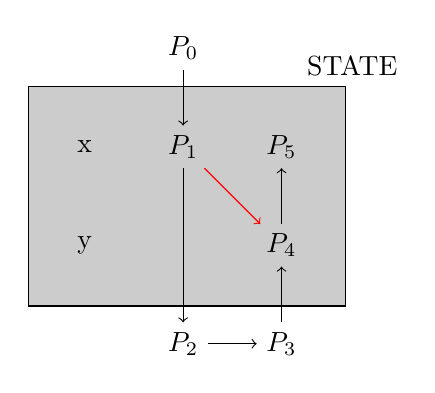
\begin{tikzpicture}[x=1.25cm,y=-1.25cm]

      \node (p0) at (0, 0) {$P_0$};
      \node (p1) at (0, 1) {$P_1$};
      \node (p2) at (0, 3) {$P_2$};
      \node (p3) at (1, 3) {$P_3$};
      \node (p4) at (1, 2) {$P_4$};
      \node (p5) at (1, 1) {$P_5$};

      \node (x) at (-1, 1) {x};
      \node (y) at (-1, 2) {y};

      \begin{pgfonlayer}{background}
        \node (q) [
          draw,
          inner sep=0.5cm,
          fill=black!20,fit=(p1) (p4) (p5) (x) (y),
          label=above right:STATE
        ] {};
      \end{pgfonlayer}

      \draw[->] (p0) -- (p1);
      \draw[->] (p1) -- (p2);
      \draw[->] (p2) -- (p3);
      \draw[->] (p3) -- (p4);
      \draw[->] (p4) -- (p5);

      \draw<2->[red,->] (p1) -- (p4);
    \end{tikzpicture}
  \end{center}

  \begin{itemize}
  \item<2->In particular: $P_1$ must not use the refined globals of $P_4$!
  \end{itemize}

\end{frame}

\begin{frame}{Phase 1}
  A global graph contains the following elements for each subprogram (and
  package elaboration):
  \begin{itemize}
  \item Locally declared variables (or parameters)
  \item Variables read
  \item Variables wrote (mode out)
  \item Remote subprograms called
  \item Remote subprograms possibly called
  \end{itemize}
\end{frame}

\begin{frame}{Phase 1}{Local calls}
  A \structure{local} call is on the same level of scope, or to an
  arbitrarily nested scope. A call from $P_1$ to $P_2$ generates the
  following links in the graph:
  \begin{itemize}
  \item $reads(P_1) \rightarrow reads(P_2)$
  \item $writes(P_1) \rightarrow writes(P_2)$
  \item $calls(P_1) \rightarrow calls(P_2)$
  \item $maybe(P_1) \rightarrow maybe(P_2)$
  \end{itemize}

  A \structure{local} maybe call from $P_1$ to $P_2$ generates the
  following links in the graph:
  \begin{itemize}
  \item $reads(P_1) \rightarrow \{reads(P_2), writes(P_2)\}$
  \item $writes(P_1) \rightarrow writes(P_2)$
  \item $maybe(P_1) \rightarrow \{calls(P_2), maybe(P_2)\}$
  \end{itemize}
\end{frame}

\begin{frame}{Phase 1}{Remote calls}
  A \structure{remote} call is anything a local call is not; i.e. to a
  different package or a call to an enclosing scope. A call from $P$ to $R$
  generates the following links in the graph:
  \begin{itemize}
  \item $calls(P) \rightarrow R$
  \end{itemize}

  A \structure{remote} maybe call from $P$ to $R$ generates the following
  links in the graph:
  \begin{itemize}
  \item $maybe(P) \rightarrow R$
  \end{itemize}
\end{frame}


\end{document}
